\section{System Design and Walkthrough}
\label{sec:system}
\subsection{Selection and interpretation}
The board contains 69 symbols in nine categories, with English, Hindi, Gujarati, and Marathi labels.
The user chooses a language, adds symbols or personal words to a sentence canvas, and may accept next-word suggestions.
Literal \emph{Speak} uses browser speech synthesis when a suitable voice exists; \emph{AI Polish \& Speak} requests sentence realization.
Quick Express, saved selections, replay, contrast, and text-size controls support repeated use; no AAC-user evaluation was conducted.

\begin{figure*}[t]
\centering
\begin{tikzpicture}[>=Stealth, node distance=5mm,
box/.style={draw=exampleblue,rounded corners=2pt,fill=panelgray,align=center,font=\small,minimum height=10mm,text width=31mm,inner sep=4pt},
check/.style={box,draw=examplegreen,fill=examplegreen!4},
edge/.style={->,thick,draw=exampleblue}]
\node[box] (input) {Symbols + language\\act + polarity};
\node[box,right=of input] (ledger) {Concept ledger\\required / forbidden};
\node[box,right=of ledger] (model) {Prompted cascade\\candidate sentence};
\node[check,right=of model] (gate) {Concept / act / polarity\\perspective / additions};
\node[box,below=9mm of input] (ask) {Ambiguous: clarify\\unsupported: preview};
\node[box,below=9mm of ledger] (template) {Language template\\checked before use};
\node[box,below=9mm of model] (output) {Labelled returned text\\model / template};
\node[box,below=9mm of gate] (speech) {Configured speech route\\or labelled test tone};
\draw[edge] (input)--(ledger);\draw[edge] (ledger)--(model);\draw[edge] (model)--(gate);
\draw[edge] (input)--(ask);
\draw[edge] (gate.south west)--node[above,sloped,font=\scriptsize]{pass}(output.north east);
\draw[edge] (gate.north) to[bend right=25] node[above,font=\scriptsize]{reject: one retry}(model.north);
\draw[edge] (template)--node[above,font=\scriptsize]{if valid}(output);
\draw[edge] (output)--(speech);
\draw[edge] (ledger)--(template);
\end{tikzpicture}

\caption{Revised decision path. The selected concepts, act, and polarity form the ledger. Model candidates and template fallbacks both pass through the checker. Clarification and literal preview do not initiate automatic speech. Prediction is a separate suggestion path; the speech route depends on installed weights or browser voices.}
\label{fig:arch}
\end{figure*}

The archived client guessed intent from substrings in the displayed labels.
It treated most selections as requests, recognized a few feeling labels, and detected negation even inside unrelated words.
The revised client instead uses board-concept identities and categories, carries act and negation separately, and offers a message-type control.
An explicit user choice takes precedence over automatic interpretation.
For an unresolved selection, clarification precedes sentence generation; an unsupported determinate selection receives a labelled literal preview rather than an inferred sentence (Figure~\ref{fig:arch}).

\subsection{Ledger, generation, and acceptance}
The ledger specifies the speaker, selected concepts, communicative act, and polarity, together with unselected content to reject.
The archived ledger forbids 21 default time, meal, and venue expressions unless selected.
Three prompted roles share one frozen \model{} model: realization, refinement, and advisory verification.
The Indic realizer has 12 Hindi, nine Gujarati, and nine Marathi examples and uses greedy decoding; English uses sampling at temperature 0.1.
The refiner is skipped for Indic-script candidates.
The verifier may suggest a rewrite, but its verdict alone cannot authorize the output.

Let $E$ be the selected concepts, $a$ the act, $\nu$ the polarity, $F$ the forbidden expressions, and $y$ a candidate.
The archived acceptance rule is
\begin{equation}
\begin{split}
A_0(y)={}& C(E,y)\land N(\nu,y)\land I_0(a,y)\\
&\land\neg B(F,y)\land\neg T(E,y).
\end{split}
\label{eq:gate}
\end{equation}
$C$ matches selected labels using substring, plural, and Indic-stem rules; $N$ matches listed negators; $I_0$ applies English feeling and question patterns; $B$ detects forbidden words; and $T$ detects unselected time expressions.
Thus the intended contract is broader than the archived checks actually enforce: first-person perspective and all possible additions are not guaranteed by Equation~\ref{eq:gate}.

The revised checker uses multilingual concept forms, act patterns, speaker-perspective patterns, and checks for additional board concepts or unrequested reasons and times.
It rejects a feeling expressed as a want and distinguishes the user's refusal from a model's refusal to answer.
These remain finite lexical checks; a candidate can match them while using an unnatural or wrong-sense construction.
A rejection permits one further cascade attempt.
After two rejected candidates, the revised policy composes a language-specific template and checks it as well.
If the template fails or no frame applies, the interface returns literal words without automatic speech.
The archived policy returned its fallback without this second check.

\subsection{Fallbacks, prediction, and speech}
Templates separately realize requests, refusals, feelings, negated feelings, action--object selections, and calls for a person.
For \lang{Hindi}, a negated feeling uses a state predicate with \hi{नहीं}; \lang{Gujarati} uses forms such as \gu{નથી}; \lang{Marathi} uses \hi{नाही} for states and \hi{नको} in refusals.
These are authored lexical resources, not independently validated language rules.
Figure~\ref{fig:ui} shows the revised clarification and fallback states, and Appendix~\ref{app:trace} shows recorded language-specific decisions.

\begin{figure}[t]
\centering
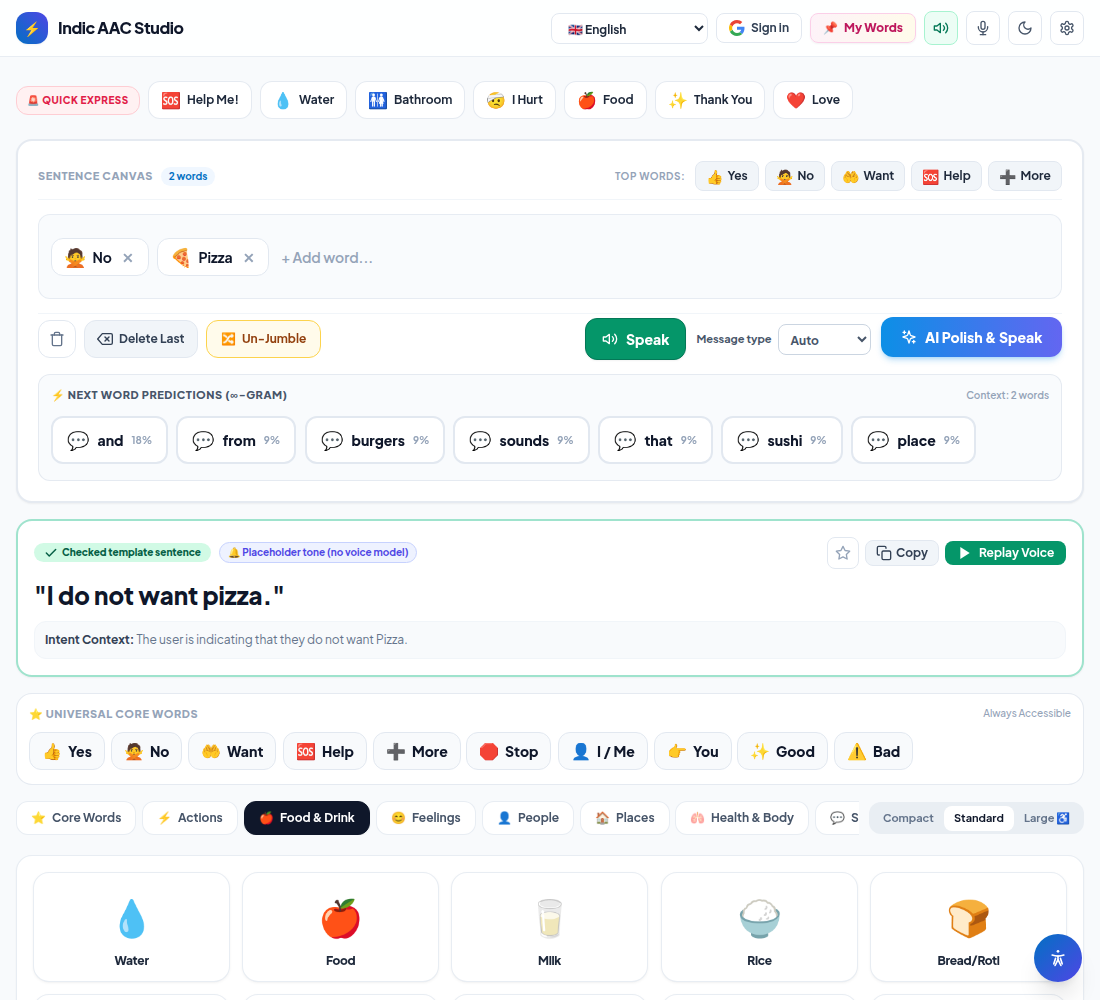
\includegraphics[width=\columnwidth,trim=20bp 340bp 640bp 510bp,clip]{figures/ui_fallback.png}\\[4pt]
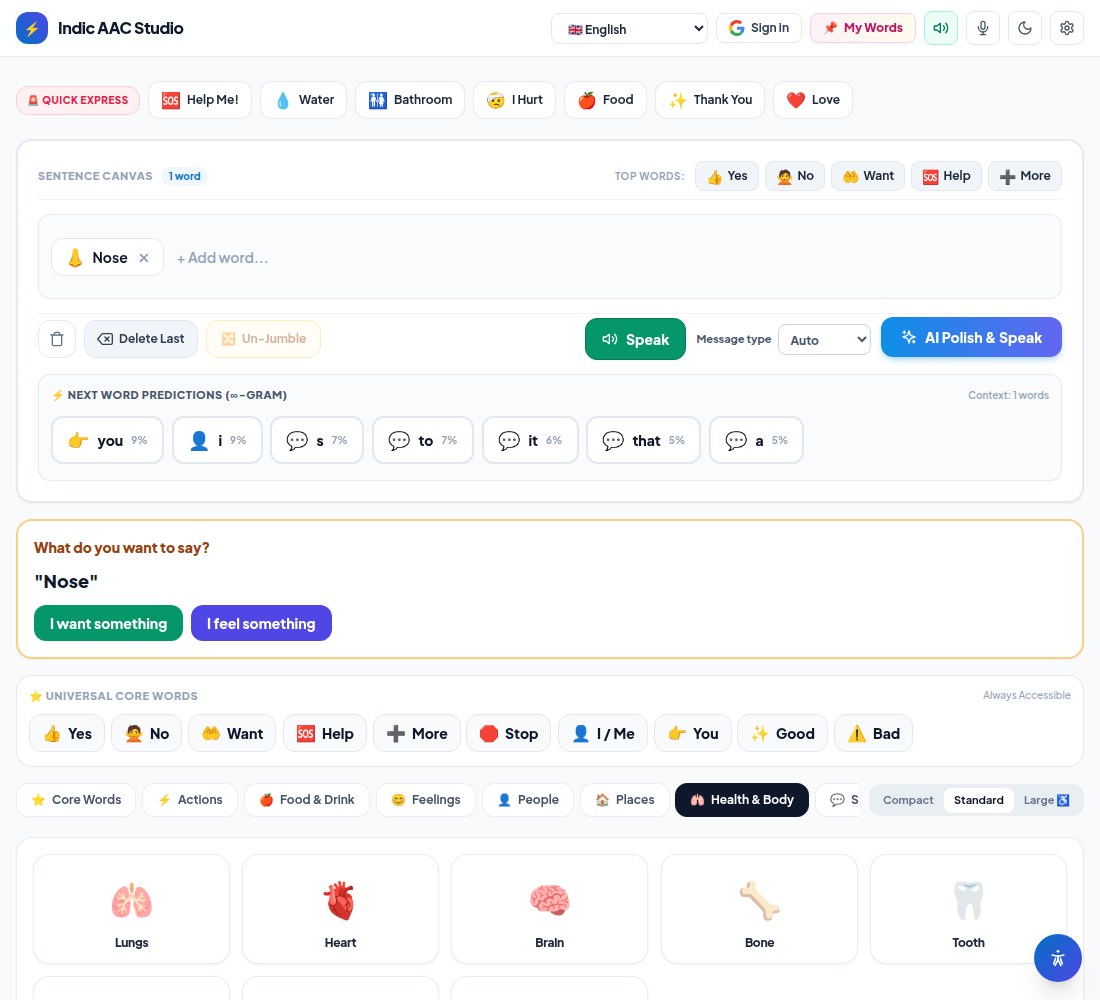
\includegraphics[width=\columnwidth,trim=20bp 340bp 640bp 510bp,clip]{figures/ui_clarification.png}
\caption{Recorded revised interface: (top detail) a rejected candidate leads to a labelled checked-template output; (bottom detail) an ambiguous selection asks the user to choose an act. The captured build labels its unavailable speech output as a 440 Hz test tone.}
\label{fig:ui}
\end{figure}

Next-word suggestions use an unbounded-order suffix trie inspired by infini-gram \citep{liu2024infinigram}, with suffix backoff weight 0.4.
The deployed trie contains 15,505 English and Hindi AAC-dialogue sentences and permits contexts up to depth 181.
Only English and Hindi have evaluated predictors; Gujarati returns English suggestions and Marathi reuses the Hindi trie.
Optional hidden Markov model (HMM) predictors and word reordering lack the required checkpoints in the evaluated build.
They therefore contribute no evidence to the sentence-generation comparison.

The configured neural speech route is \emph{IndicF5}, with a 24\,kHz \emph{Vocos} vocoder and reference-audio conditioning \citep{ai4bharat2025indicf5,siuzdak2023vocos}.
The IndicF5 model card lists Hindi, Gujarati, and Marathi among 11 supported languages, but does not list English.
The implementation nevertheless selects an English reference for English and an Indic reference for the other three languages; this routing is not evidence of successful synthesis.
The audited machines lacked the gated IndicF5 weights, all measured playback was a 440 Hz test tone, and headless Chrome exposed no browser voices.
Accordingly, the verified scope of this paper is sentence generation and playback integration, rather than audible four-language speech.
